\documentclass{article}
\usepackage[utf8]{inputenc}
\usepackage{amssymb}
\usepackage{listings}
\usepackage{graphicx}


\title{The Exponential Function}
\author{Emil Lenler-Eriksen}
\date{May 2022}

\begin{document}

\maketitle
The exponential function is a function taking some complex number $x$ and returning a function value as proscribed by: $$f(x) : x \rightarrow e^x $$
Where $e$ is Euler's number. The function has been applied to a wide range of fields including biology, economy, physics and of course mathematics as well. One of the key characteristics of the exponential function is that its derivative at some point $x$ is equal to the value of the function itself in that same point. That is $\frac{d}{dx}e^x = e^x$. This feature of the exponential function is perhaps most easily seen when one considers the Taylor series of the function, which is given as:
\begin{equation}
    e^x = \sum_{n = 0}^\infty \frac{x^n}{n!}
\end{equation}
Due to the wide range of applicability of the function in mathematical models for all kinds of systems it is important to have efficient numerical implementations of the exponential function. One example of a very basic numerical implementation of the exponential function (accepting real valued $x$) in C\# might be:
\begin{lstlisting}
static double ex(double x){
        (i) if(x<0)return 1/ex(-x);
        (ii) if(x>1.0/8)return Pow(ex(x/2),2);
        (iii) return 1+x*(1+x/2*(1+x/3*(1+x/4*(1+x/5*(1+x/6...
        *(1+x/7*(1+x/8*(1+x/9*(1+x/10)))))))));
}
\end{lstlisting}
where the ellipses simply denote that the line is continued below and the roman numerals at the beginning of each line are there for reference purposes.\\
The first line (i) is there for the purposes of dealing with negative values of $x$. By the "regular" rules of exponentiation we simply compute the value of $e^{\vert x \vert}$ and take the reciprocal value. Line (ii) relates to line (iii) when we actually compute the value we do so by computing the first few terms of the Taylor series. As such this expression is only valid for $x\ll1$, however we wish to perform the value for arbitrary $x$. We thus work around it by writing the code recursively, calculating the exponential for $x/2$ and then squaring it if $x$ is too large. Finally line (iii) just computes the Taylor series up to the 10'th order term.
The implementation above has been carried out and compared to the built-in exponential function in C\# producing figure 1.\\
\begin{figure}
    \centering
    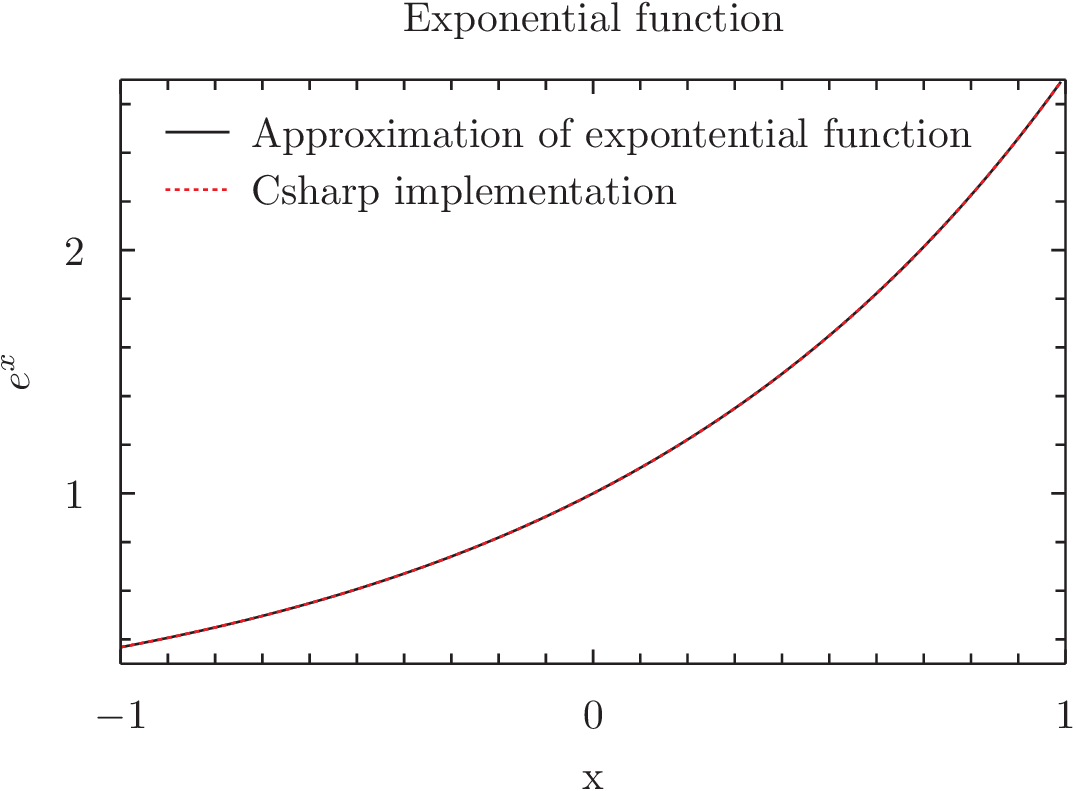
\includegraphics{plot.png}
    \caption{Comparison of "primitive" implementation of exponential function and built-in C\# implementation}
    \label{fig:my_label}
\end{figure}
\end{document}